%********************************************%
%*       Generated from PreTeXt source      *%
%*       on 2021-12-06T19:03:29Z       *%
%*   A recent stable commit (2020-08-09):   *%
%* 98f21740783f166a773df4dc83cab5293ab63a4a *%
%*                                          *%
%*         https://pretextbook.org          *%
%*                                          *%
%********************************************%
%% We elect to always write snapshot output into <job>.dep file
\RequirePackage{snapshot}
\documentclass[oneside,10pt,]{article}
%% Custom Preamble Entries, early (use latex.preamble.early)
%% Default LaTeX packages
%%   1.  always employed (or nearly so) for some purpose, or
%%   2.  a stylewriter may assume their presence
\usepackage{geometry}
%% Some aspects of the preamble are conditional,
%% the LaTeX engine is one such determinant
\usepackage{ifthen}
%% etoolbox has a variety of modern conveniences
\usepackage{etoolbox}
\usepackage{ifxetex,ifluatex}
%% Raster graphics inclusion
\usepackage{graphicx}
%% Color support, xcolor package
%% Always loaded, for: add/delete text, author tools
%% Here, since tcolorbox loads tikz, and tikz loads xcolor
\PassOptionsToPackage{usenames,dvipsnames,svgnames,table}{xcolor}
\usepackage{xcolor}
%% begin: defined colors, via xcolor package, for styling
%% end: defined colors, via xcolor package, for styling
%% Colored boxes, and much more, though mostly styling
%% skins library provides "enhanced" skin, employing tikzpicture
%% boxes may be configured as "breakable" or "unbreakable"
%% "raster" controls grids of boxes, aka side-by-side
\usepackage{tcolorbox}
\tcbuselibrary{skins}
\tcbuselibrary{breakable}
\tcbuselibrary{raster}
%% We load some "stock" tcolorbox styles that we use a lot
%% Placement here is provisional, there will be some color work also
%% First, black on white, no border, transparent, but no assumption about titles
\tcbset{ bwminimalstyle/.style={size=minimal, boxrule=-0.3pt, frame empty,
colback=white, colbacktitle=white, coltitle=black, opacityfill=0.0} }
%% Second, bold title, run-in to text/paragraph/heading
%% Space afterwards will be controlled by environment,
%% independent of constructions of the tcb title
%% Places \blocktitlefont onto many block titles
\tcbset{ runintitlestyle/.style={fonttitle=\blocktitlefont\upshape\bfseries, attach title to upper} }
%% Spacing prior to each exercise, anywhere
\tcbset{ exercisespacingstyle/.style={before skip={1.5ex plus 0.5ex}} }
%% Spacing prior to each block
\tcbset{ blockspacingstyle/.style={before skip={2.0ex plus 0.5ex}} }
%% xparse allows the construction of more robust commands,
%% this is a necessity for isolating styling and behavior
%% The tcolorbox library of the same name loads the base library
\tcbuselibrary{xparse}
%% Hyperref should be here, but likes to be loaded late
%%
%% Inline math delimiters, \(, \), need to be robust
%% 2016-01-31:  latexrelease.sty  supersedes  fixltx2e.sty
%% If  latexrelease.sty  exists, bugfix is in kernel
%% If not, bugfix is in  fixltx2e.sty
%% See:  https://tug.org/TUGboat/tb36-3/tb114ltnews22.pdf
%% and read "Fewer fragile commands" in distribution's  latexchanges.pdf
\IfFileExists{latexrelease.sty}{}{\usepackage{fixltx2e}}
%% Text height identically 9 inches, text width varies on point size
%% See Bringhurst 2.1.1 on measure for recommendations
%% 75 characters per line (count spaces, punctuation) is target
%% which is the upper limit of Bringhurst's recommendations
\geometry{letterpaper,total={340pt,9.0in}}
%% Custom Page Layout Adjustments (use latex.geometry)
%% This LaTeX file may be compiled with pdflatex, xelatex, or lualatex executables
%% LuaTeX is not explicitly supported, but we do accept additions from knowledgeable users
%% The conditional below provides  pdflatex  specific configuration last
%% begin: engine-specific capabilities
\ifthenelse{\boolean{xetex} \or \boolean{luatex}}{%
%% begin: xelatex and lualatex-specific default configuration
\ifxetex\usepackage{xltxtra}\fi
%% realscripts is the only part of xltxtra relevant to lualatex 
\ifluatex\usepackage{realscripts}\fi
%% end:   xelatex and lualatex-specific default configuration
}{
%% begin: pdflatex-specific default configuration
%% We assume a PreTeXt XML source file may have Unicode characters
%% and so we ask LaTeX to parse a UTF-8 encoded file
%% This may work well for accented characters in Western language,
%% but not with Greek, Asian languages, etc.
%% When this is not good enough, switch to the  xelatex  engine
%% where Unicode is better supported (encouraged, even)
\usepackage[utf8]{inputenc}
%% end: pdflatex-specific default configuration
}
%% end:   engine-specific capabilities
%%
%% Fonts.  Conditional on LaTex engine employed.
%% Default Text Font: The Latin Modern fonts are
%% "enhanced versions of the [original TeX] Computer Modern fonts."
%% We use them as the default text font for PreTeXt output.
%% Default Monospace font: Inconsolata (aka zi4)
%% Sponsored by TUG: http://levien.com/type/myfonts/inconsolata.html
%% Loaded for documents with intentional objects requiring monospace
%% See package documentation for excellent instructions
%% fontspec will work universally if we use filename to locate OTF files
%% Loads the "upquote" package as needed, so we don't have to
%% Upright quotes might come from the  textcomp  package, which we also use
%% We employ the shapely \ell to match Google Font version
%% pdflatex: "varl" package option produces shapely \ell
%% pdflatex: "var0" package option produces plain zero (not used)
%% pdflatex: "varqu" package option produces best upright quotes
%% xelatex,lualatex: add OTF StylisticSet 1 for shapely \ell
%% xelatex,lualatex: add OTF StylisticSet 2 for plain zero (not used)
%% xelatex,lualatex: add OTF StylisticSet 3 for upright quotes
%%
%% Automatic Font Control
%% Portions of a document, are, or may, be affected by defined commands
%% These are perhaps more flexible when using  xelatex  rather than  pdflatex
%% The following definitions are meant to be re-defined in a style, using \renewcommand
%% They are scoped when employed (in a TeX group), and so should not be defined with an argument
\newcommand{\divisionfont}{\relax}
\newcommand{\blocktitlefont}{\relax}
\newcommand{\contentsfont}{\relax}
\newcommand{\pagefont}{\relax}
\newcommand{\tabularfont}{\relax}
\newcommand{\xreffont}{\relax}
\newcommand{\titlepagefont}{\relax}
%%
\ifthenelse{\boolean{xetex} \or \boolean{luatex}}{%
%% begin: font setup and configuration for use with xelatex
%% Generally, xelatex is necessary for non-Western fonts
%% fontspec package provides extensive control of system fonts,
%% meaning *.otf (OpenType), and apparently *.ttf (TrueType)
%% that live *outside* your TeX/MF tree, and are controlled by your *system*
%% (it is possible that a TeX distribution will place fonts in a system location)
%%
%% The fontspec package is the best vehicle for using different fonts in  xelatex
%% So we load it always, no matter what a publisher or style might want
%%
\usepackage{fontspec}
%%
%% begin: xelatex main font ("font-xelatex-main" template)
%% Latin Modern Roman is the default font for xelatex and so is loaded with a TU encoding
%% *in the format* so we can't touch it, only perhaps adjust it later
%% in one of two ways (then known by NFSS names such as "lmr")
%% (1) via NFSS with font family names such as "lmr" and "lmss"
%% (2) via fontspec with commands like \setmainfont{Latin Modern Roman}
%% The latter requires the font to be known at the system-level by its font name,
%% but will give access to OTF font features through optional arguments
%% https://tex.stackexchange.com/questions/470008/
%% where-and-how-does-fontspec-sty-specify-the-default-font-latin-modern-roman
%% http://tex.stackexchange.com/questions/115321
%% /how-to-optimize-latin-modern-font-with-xelatex
%%
%% end:   xelatex main font ("font-xelatex-main" template)
%% begin: xelatex mono font ("font-xelatex-mono" template)
%% (conditional on non-trivial uses being present in source)
\IfFontExistsTF{Inconsolatazi4-Regular.otf}{}{\GenericError{}{The font "Inconsolatazi4-Regular.otf" requested by PreTeXt output is not available.  Either a file cannot be located in default locations via a filename, or a font is not known by its name as part of your system.}{Consult the PreTeXt Guide for help with LaTeX fonts.}{}}
\IfFontExistsTF{Inconsolatazi4-Bold.otf}{}{\GenericError{}{The font "Inconsolatazi4-Bold.otf" requested by PreTeXt output is not available.  Either a file cannot be located in default locations via a filename, or a font is not known by its name as part of your system.}{Consult the PreTeXt Guide for help with LaTeX fonts.}{}}
\usepackage{zi4}
\setmonofont[BoldFont=Inconsolatazi4-Bold.otf,StylisticSet={1,3}]{Inconsolatazi4-Regular.otf}
%% end:   xelatex mono font ("font-xelatex-mono" template)
%% begin: xelatex font adjustments ("font-xelatex-style" template)
%% end:   xelatex font adjustments ("font-xelatex-style" template)
%%
%% Extensive support for other languages
\usepackage{polyglossia}
%% Set main/default language based on pretext/@xml:lang value
%% document language code is "en-US", US English
%% usmax variant has extra hypenation
\setmainlanguage[variant=usmax]{english}
%% Enable secondary languages based on discovery of @xml:lang values
%% Enable fonts/scripts based on discovery of @xml:lang values
%% Western languages should be ably covered by Latin Modern Roman
%% end:   font setup and configuration for use with xelatex
}{%
%% begin: font setup and configuration for use with pdflatex
%% begin: pdflatex main font ("font-pdflatex-main" template)
\usepackage{lmodern}
\usepackage[T1]{fontenc}
%% end:   pdflatex main font ("font-pdflatex-main" template)
%% begin: pdflatex mono font ("font-pdflatex-mono" template)
%% (conditional on non-trivial uses being present in source)
\usepackage[varqu,varl]{inconsolata}
%% end:   pdflatex mono font ("font-pdflatex-mono" template)
%% begin: pdflatex font adjustments ("font-pdflatex-style" template)
%% end:   pdflatex font adjustments ("font-pdflatex-style" template)
%% end:   font setup and configuration for use with pdflatex
}
%% Micromanage spacing, etc.  The named "microtype-options"
%% template may be employed to fine-tune package behavior
\usepackage{microtype}
%% Symbols, align environment, commutative diagrams, bracket-matrix
\usepackage{amsmath}
\usepackage{amscd}
\usepackage{amssymb}
%% allow page breaks within display mathematics anywhere
%% level 4 is maximally permissive
%% this is exactly the opposite of AMSmath package philosophy
%% there are per-display, and per-equation options to control this
%% split, aligned, gathered, and alignedat are not affected
\allowdisplaybreaks[4]
%% allow more columns to a matrix
%% can make this even bigger by overriding with  latex.preamble.late  processing option
\setcounter{MaxMatrixCols}{30}
%%
%%
%% Division Titles, and Page Headers/Footers
%% titlesec package, loading "titleps" package cooperatively
%% See code comments about the necessity and purpose of "explicit" option.
%% The "newparttoc" option causes a consistent entry for parts in the ToC 
%% file, but it is only effective if there is a \titleformat for \part.
%% "pagestyles" loads the  titleps  package cooperatively.
\usepackage[explicit, newparttoc, pagestyles]{titlesec}
%% The companion titletoc package for the ToC.
\usepackage{titletoc}
%% begin: customizations of page styles via the modal "titleps-style" template
%% Designed to use commands from the LaTeX "titleps" package
\pagestyle{plain}
%% end: customizations of page styles via the modal "titleps-style" template
%%
%% Create globally-available macros to be provided for style writers
%% These are redefined for each occurence of each division
\newcommand{\divisionnameptx}{\relax}%
\newcommand{\titleptx}{\relax}%
\newcommand{\subtitleptx}{\relax}%
\newcommand{\shortitleptx}{\relax}%
\newcommand{\authorsptx}{\relax}%
\newcommand{\epigraphptx}{\relax}%
%% Create environments for possible occurences of each division
%% Environment for a PTX "section" at the level of a LaTeX "section"
\NewDocumentEnvironment{sectionptx}{mmmmmm}
{%
\renewcommand{\divisionnameptx}{Section}%
\renewcommand{\titleptx}{#1}%
\renewcommand{\subtitleptx}{#2}%
\renewcommand{\shortitleptx}{#3}%
\renewcommand{\authorsptx}{#4}%
\renewcommand{\epigraphptx}{#5}%
\section[{#3}]{#1}%
\label{#6}%
}{}%
%% Environment for a PTX "subsection" at the level of a LaTeX "subsection"
\NewDocumentEnvironment{subsectionptx}{mmmmmm}
{%
\renewcommand{\divisionnameptx}{Subsection}%
\renewcommand{\titleptx}{#1}%
\renewcommand{\subtitleptx}{#2}%
\renewcommand{\shortitleptx}{#3}%
\renewcommand{\authorsptx}{#4}%
\renewcommand{\epigraphptx}{#5}%
\subsection[{#3}]{#1}%
\label{#6}%
}{}%
%% Environment for a PTX "references" at the level of a LaTeX "section"
\NewDocumentEnvironment{references-section}{mmmmmm}
{%
\renewcommand{\divisionnameptx}{References}%
\renewcommand{\titleptx}{#1}%
\renewcommand{\subtitleptx}{#2}%
\renewcommand{\shortitleptx}{#3}%
\renewcommand{\authorsptx}{#4}%
\renewcommand{\epigraphptx}{#5}%
\section[{#3}]{#1}%
\label{#6}%
}{}%
%% Environment for a PTX "references" at the level of a LaTeX "section"
\NewDocumentEnvironment{references-section-numberless}{mmmmmm}
{%
\renewcommand{\divisionnameptx}{References}%
\renewcommand{\titleptx}{#1}%
\renewcommand{\subtitleptx}{#2}%
\renewcommand{\shortitleptx}{#3}%
\renewcommand{\authorsptx}{#4}%
\renewcommand{\epigraphptx}{#5}%
\section*{#1}%
\addcontentsline{toc}{section}{#3}
\label{#6}%
}{}%
%%
%% Styles for six traditional LaTeX divisions
\titleformat{\part}[display]
{\divisionfont\Huge\bfseries\centering}{\divisionnameptx\space\thepart}{30pt}{\Huge#1}
[{\Large\centering\authorsptx}]
\titleformat{\chapter}[display]
{\divisionfont\huge\bfseries}{\divisionnameptx\space\thechapter}{20pt}{\Huge#1}
[{\Large\authorsptx}]
\titleformat{name=\chapter,numberless}[display]
{\divisionfont\huge\bfseries}{}{0pt}{#1}
[{\Large\authorsptx}]
\titlespacing*{\chapter}{0pt}{50pt}{40pt}
\titleformat{\section}[hang]
{\divisionfont\Large\bfseries}{\thesection}{1ex}{#1}
[{\large\authorsptx}]
\titleformat{name=\section,numberless}[block]
{\divisionfont\Large\bfseries}{}{0pt}{#1}
[{\large\authorsptx}]
\titlespacing*{\section}{0pt}{3.5ex plus 1ex minus .2ex}{2.3ex plus .2ex}
\titleformat{\subsection}[hang]
{\divisionfont\large\bfseries}{\thesubsection}{1ex}{#1}
[{\normalsize\authorsptx}]
\titleformat{name=\subsection,numberless}[block]
{\divisionfont\large\bfseries}{}{0pt}{#1}
[{\normalsize\authorsptx}]
\titlespacing*{\subsection}{0pt}{3.25ex plus 1ex minus .2ex}{1.5ex plus .2ex}
\titleformat{\subsubsection}[hang]
{\divisionfont\normalsize\bfseries}{\thesubsubsection}{1em}{#1}
[{\small\authorsptx}]
\titleformat{name=\subsubsection,numberless}[block]
{\divisionfont\normalsize\bfseries}{}{0pt}{#1}
[{\normalsize\authorsptx}]
\titlespacing*{\subsubsection}{0pt}{3.25ex plus 1ex minus .2ex}{1.5ex plus .2ex}
\titleformat{\paragraph}[hang]
{\divisionfont\normalsize\bfseries}{\theparagraph}{1em}{#1}
[{\small\authorsptx}]
\titleformat{name=\paragraph,numberless}[block]
{\divisionfont\normalsize\bfseries}{}{0pt}{#1}
[{\normalsize\authorsptx}]
\titlespacing*{\paragraph}{0pt}{3.25ex plus 1ex minus .2ex}{1.5em}
%%
%% Styles for five traditional LaTeX divisions
\titlecontents{part}%
[0pt]{\contentsmargin{0em}\addvspace{1pc}\contentsfont\bfseries}%
{\Large\thecontentslabel\enspace}{\Large}%
{}%
[\addvspace{.5pc}]%
\titlecontents{chapter}%
[0pt]{\contentsmargin{0em}\addvspace{1pc}\contentsfont\bfseries}%
{\large\thecontentslabel\enspace}{\large}%
{\hfill\bfseries\thecontentspage}%
[\addvspace{.5pc}]%
\dottedcontents{section}[3.8em]{\contentsfont}{2.3em}{1pc}%
\dottedcontents{subsection}[6.1em]{\contentsfont}{3.2em}{1pc}%
\dottedcontents{subsubsection}[9.3em]{\contentsfont}{4.3em}{1pc}%
%%
%% Begin: Semantic Macros
%% To preserve meaning in a LaTeX file
%%
%% \mono macro for content of "c", "cd", "tag", etc elements
%% Also used automatically in other constructions
%% Simply an alias for \texttt
%% Always defined, even if there is no need, or if a specific tt font is not loaded
\newcommand{\mono}[1]{\texttt{#1}}
%%
%% Following semantic macros are only defined here if their
%% use is required only in this specific document
%%
%% Used for inline definitions of terms
\newcommand{\terminology}[1]{\textbf{#1}}
%% End: Semantic Macros
%% Localize LaTeX supplied names (possibly none)
\renewcommand*{\abstractname}{Abstract}
%% "tcolorbox" environment for a single image, occupying entire \linewidth
%% arguments are left-margin, width, right-margin, as multiples of
%% \linewidth, and are guaranteed to be positive and sum to 1.0
\tcbset{ imagestyle/.style={bwminimalstyle} }
\NewTColorBox{image}{mmm}{imagestyle,left skip=#1\linewidth,width=#2\linewidth}
%% More flexible list management, esp. for references
%% But also for specifying labels (i.e. custom order) on nested lists
\usepackage{enumitem}
%% Lists of references in their own section, maximum depth 1
\newlist{referencelist}{description}{4}
\setlist[referencelist]{leftmargin=!,labelwidth=!,labelsep=0ex,itemsep=1.0ex,topsep=1.0ex,partopsep=0pt,parsep=0pt}
%% hyperref driver does not need to be specified, it will be detected
%% Footnote marks in tcolorbox have broken linking under
%% hyperref, so it is necessary to turn off all linking
%% It *must* be given as a package option, not with \hypersetup
\usepackage[hyperfootnotes=false]{hyperref}
%% configure hyperref's  \url  to match listings' inline verbatim
\renewcommand\UrlFont{\small\ttfamily}
%% Hyperlinking active in electronic PDFs, all links solid and blue
\hypersetup{colorlinks=true,linkcolor=blue,citecolor=blue,filecolor=blue,urlcolor=blue}
\hypersetup{pdftitle={Open Technologies for Undergraduate Mathematics Education}}
%% If you manually remove hyperref, leave in this next command
%% This will allow LaTeX compilation, employing this no-op command
\providecommand\phantomsection{}
%% Division Numbering: Chapters, Sections, Subsections, etc
%% Division numbers may be turned off at some level ("depth")
%% A section *always* has depth 1, contrary to us counting from the document root
%% The latex default is 3.  If a larger number is present here, then
%% removing this command may make some cross-references ambiguous
%% The precursor variable $numbering-maxlevel is checked for consistency in the common XSL file
\setcounter{secnumdepth}{3}
%%
%% AMS "proof" environment is no longer used, but we leave previously
%% implemented \qedhere in place, should the LaTeX be recycled
\newcommand{\qedhere}{\relax}
%%
%% A faux tcolorbox whose only purpose is to provide common numbering
%% facilities for most blocks (possibly not projects, 2D displays)
%% Controlled by  numbering.theorems.level  processing parameter
\newtcolorbox[auto counter, number within=section]{block}{}
%%
%% This document is set to number PROJECT-LIKE on a separate numbering scheme
%% So, a faux tcolorbox whose only purpose is to provide this numbering
%% Controlled by  numbering.projects.level  processing parameter
\newtcolorbox[auto counter, number within=section]{project-distinct}{}
%% A faux tcolorbox whose only purpose is to provide common numbering
%% facilities for 2D displays which are subnumbered as part of a "sidebyside"
\makeatletter
\newtcolorbox[auto counter, number within=tcb@cnt@block, number freestyle={\noexpand\thetcb@cnt@block(\noexpand\alph{\tcbcounter})}]{subdisplay}{}
\makeatother
%%
%% tcolorbox, with styles, for FIGURE-LIKE
%%
%% figureptx: 2-D display structure
\tcbset{ figureptxstyle/.style={bwminimalstyle, middle=1ex, blockspacingstyle, fontlower=\blocktitlefont} }
\newtcolorbox[use counter from=block]{figureptx}[3]{lower separated=false, before lower={{\textbf{Figure~\thetcbcounter}\space#1}}, phantomlabel={#2}, unbreakable, parbox=false, figureptxstyle, }
%%
%% xparse environments for introductions and conclusions of divisions
%%
%% introduction: in a structured division
\NewDocumentEnvironment{introduction}{m}
{\notblank{#1}{\noindent\textbf{#1}\space}{}}{\par\medskip}
%% Graphics Preamble Entries
\usepackage{tikz}
%% If tikz has been loaded, replace ampersand with \amp macro
%% extpfeil package for certain extensible arrows,
%% as also provided by MathJax extension of the same name
%% NB: this package loads mtools, which loads calc, which redefines
%%     \setlength, so it can be removed if it seems to be in the 
%%     way and your math does not use:
%%     
%%     \xtwoheadrightarrow, \xtwoheadleftarrow, \xmapsto, \xlongequal, \xtofrom
%%     
%%     we have had to be extra careful with variable thickness
%%     lines in tables, and so also load this package late
\usepackage{extpfeil}
%% Custom Preamble Entries, late (use latex.preamble.late)
%% Begin: Author-provided packages
%% (From  docinfo/latex-preamble/package  elements)
%% End: Author-provided packages
%% Begin: Author-provided macros
%% (From  docinfo/macros  element)
%% Plus three from MBX for XML characters
\newcommand{\foo}{b^{ar}}
\newcommand{\lt}{<}
\newcommand{\gt}{>}
\newcommand{\amp}{&}
%% End: Author-provided macros
%% Title page information for article
\title{Open Technologies for Undergraduate Mathematics Education\\
{\large Application for 2022 Arts and Sciences Summer Professional Development Award}}
\author{Steven Clontz\\
Assistant Professor of Mathematics (tenure-track)\\
Department of Mathematics and Statistics\\
University of South Alabama
}
\date{2021 December}
\begin{document}
%% Target for xref to top-level element is document start
\hypertarget{x:article:sabbatical-proposal}{}
\maketitle
\thispagestyle{empty}
\begin{abstract}
NSF's Office of Advanced Cyberinfrastructure (OAC) ``supports and coordinates the development, acquisition, and provision of state-of-the-art cyberinfrastructure resources, tools and services essential to the advancement and transformation of science and engineering''. In service of this mission, Dr. Clontz serves as co-PI on NSF DUE Award 2011807 \hyperlink{x:biblio:biblio-tbil-award}{[{\xreffont 17}]}, responsible for the development of classroom materials relying on several open-source technologies built to support evidence-based pedagogies in undergraduate mathematics education.%
\par
This proposal requests to leverage the momentum from this project by allowing Clontz to extend his current NSF support to spend the full Summer 2022 term developing these technologies themselves, as well as prepare his first NSF grant proposal as Principal Investigator specifically dedicated to developing and evaluating these technologies for use in the undergraduate mathematics classroom.%
\end{abstract}
\newpage
%
%
\typeout{************************************************}
\typeout{Section 1 Background}
\typeout{************************************************}
%
\begin{sectionptx}{Background}{}{Background}{}{}{x:section:background}
\begin{introduction}{}%
The term \terminology{cyberinfrastructure} traces its roots back to Presidential Decision Directive NSC-63 \hyperlink{x:biblio:biblio-prez}{[{\xreffont 27}]}, and is commonly used today to refer to ``computational systems, data and information management, advanced instruments, visualization environments, and people, all linked together by software and advanced networks to improve scholarly productivity and enable knowledge breakthroughs and discoveries not otherwise possible'' \hyperlink{x:biblio:biblio-cyber-educause}{[{\xreffont 14}]}. What cyberinfrastructure ``looks like'' varies greatly between disciplines, but a constant quality of it is the utilization of modern technologies that make the jobs of scholars more efficient, thereby producing more and better advancements in STEM. As such, the National Science Foundation \hyperlink{x:biblio:biblio-cyber-nsf}{[{\xreffont 19}]} and other federal agencies have made the development of cyberinfrastructure a key priority in supporting STEM scholarship as noted below (emphasis added):%
\begin{quote}%
NSF invests in powerful cyberinfrastructure that enhances the ability of researchers and educators to access and use scientific data and infrastructure. These assets include high-performance computing systems, large-scale data repositories, \emph{software suites}, networks, and digital access to research equipment and instrumentation \emph{as well as education resources}. \hyperlink{x:biblio:biblio-cyber-researchgov}{[{\xreffont 23}]}%
\end{quote}
\end{introduction}%
%
%
\typeout{************************************************}
\typeout{Subsection 1.1 Cyberinfrastructure in Mathematics Instruction and RUME}
\typeout{************************************************}
%
\begin{subsectionptx}{Cyberinfrastructure in Mathematics Instruction and RUME}{}{Cyberinfrastructure in Mathematics Instruction and RUME}{}{}{g:subsection:idm139889428815032}
Logistics are frequently a limiting factor in the adoption of evidence-based practices in instruction, particularly in undergraduate mathematics education \hyperlink{x:biblio:biblio-logistics}{[{\xreffont 24}]}. Often, faculty are willing, if not eager, to change instruction in ways that benefit students, but do not have the resources to implement such change.%
\par
Likewise, the authors of \hyperlink{x:biblio:biblio-calcplot3d}{[{\xreffont 26}]} observed the limitations of educational software that technically works, but isn't designed for platforms that are readily in the hands of students and instructors. For example, while CalcPlot3D has always been free and open-source software, it was originally limited in its reach due to being written in Java. By rewriting the application in (the similarly-named but unrelated programming language) Javascript, students and instructors were no longer required to be at a computer station with a Java runtime installed, but could instead utilize the program from any device with a web browser.%
\par
To facilitate his work supported by NSF DUE 2011807, Clontz has developed two software applications to support mathematics instruction and Team-Based Inquiry Learning (TBIL), a flavor of Team-Based Learning that was the focus of the University's most recent Quality Enhancement Project. The first is the CheckIt Platform \hyperlink{x:biblio:biblio-checkit}{[{\xreffont 7}]}, allowing instructors to write minimal code to generate randomized mathematics exercises that can be automatically exported not only to LaTeX\slash{}PDF for printing, but also published to the web as practice exercises, and to LMSes including Canvas, D2L, and Moodle. The second is Scratchee \hyperlink{x:biblio:biblio-scratchee}{[{\xreffont 10}]}, a virtualization of the Instant Feedback Assessment Technique (IF-AT) \hyperlink{x:biblio:biblio-ifat}{[{\xreffont 12}]} integral to TBIL. In addition, Clontz serves as collaborator on the PreTeXt project \hyperlink{x:biblio:biblio-pretext}{[{\xreffont 5}]}, developing a user-friendly platform for authoring the PreTeXt markup language that produces both PDF and accessible HTML documents (including textbooks and research manuscripts) from the same source, including this proposal \hyperlink{x:biblio:biblio-repo}{[{\xreffont 11}]}. Furthermore, docuemnts authored in PreTeXt can also be automatically published as Braille \hyperlink{x:biblio:biblio-braille}{[{\xreffont 2}]}, an uncommon feature for commercial textbooks, much less free Open Educational Resources (OER), providing access to mathematics often out of reach to blind students.%
\begin{figureptx}{A demo CheckIt randomized exercise exportable to LaTeX, HTML, and more.}{g:figure:idm139889428807960}{}%
\begin{image}{0}{1}{0}%
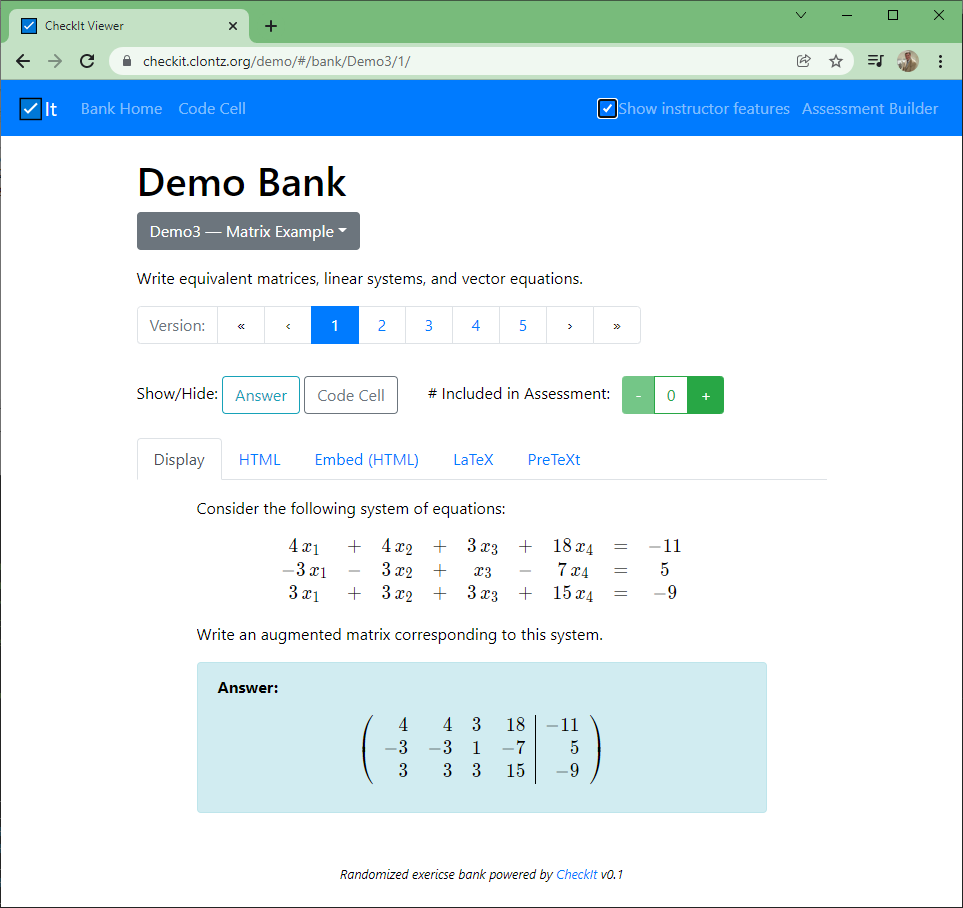
\includegraphics[width=0.9\linewidth]{external/checkit.png}
\end{image}%
\tcblower
\end{figureptx}%
\begin{figureptx}{IF-AT card designer powered by Scratchee.}{g:figure:idm139889428806712}{}%
\begin{image}{0}{1}{0}%
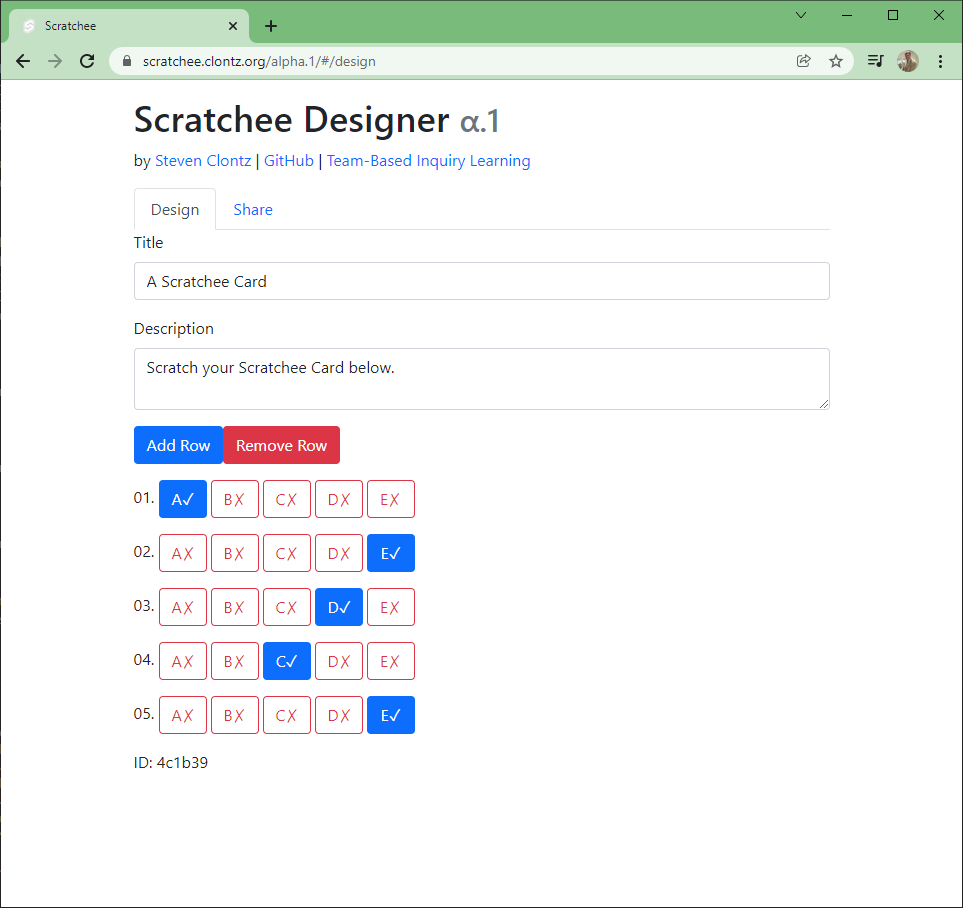
\includegraphics[width=0.9\linewidth]{external/scratchee.png}
\end{image}%
\tcblower
\end{figureptx}%
In addition to supporting mathematics instruction directly, the CheckIt Platform is also being used to support Research in Undergraduate Mathematics Education (RUME). Exercises on the platform are designed to assess particular learning outcomes; in order to measure the effectiveness of instruction as part of DUE 2011807, CheckIt-generated assessments will be used at several campuses across the country. This allows instructors to administer as many versions of each exercise as needed for logistical purposes, while still ensuring that each version of the exercise measures exactly the same learning outcome.%
\par
Finally, the development of Checkit itself raises several interesting RUME questions that Clontz aims to explore in future collaborations with education researchers. For example, the process of authoring an exercise that aims to assess a particular learning outcome is much simpler than authoring an exercise template to be seeded with randomized data. In mathematics this is sometimes achievable by simply randomizing numerical elements of the exercise; for example, the template \mono{\{\{a\}\}x + \{\{b\}\}y = \{\{c\}\}} expressing the standard equation of a line might be randomized to \(4x+5y=-2\), \(-3x+y=0\), and so on. However, what constraints are appropriate for this randomization to ensure it still serves as a valid assessment of a given outcome? Certainly, it seems unlikely that examples such as \(531284127x-4512874312y=341893123\) are necessary. But should the line occassionally be expressed in point-slope form \(y=-mx+b\) instead? And how can the stem of a question be randomized to ensure that students are synthesizing complete instructions, rather than only memorizing patterns developed from seeing solutions to similarly-generated exercises?%
\end{subsectionptx}
%
%
\typeout{************************************************}
\typeout{Subsection 1.2 Free and Open-Source Software (FOSS)}
\typeout{************************************************}
%
\begin{subsectionptx}{Free and Open-Source Software (FOSS)}{}{Free and Open-Source Software (FOSS)}{}{}{g:subsection:idm139889428801688}
The focus of this project is on \terminology{Free and Open-Source Software} that will benefit undergraduate students and instructors of mathematics. Generally, the NSF requires that software products it funds be FOSS. It's worth clarifying what is meant by this.%
\par
\terminology{Open-source software} is most easily defined. All code written as part of this project will be made available to the public via Clontz's GitHub \hyperlink{x:biblio:biblio-ghclontz}{[{\xreffont 9}]} (or other publicly available repositories as appropriate). This means that anyone will be able to obtain a copy of any software developed during this sabbatical, use this software to benefit their research or instruction, and contribute corrections or improvements to the codebase to benefit others.%
\par
The word \terminology{free} in FOSS does the heaviest lifting. Primarily, it means that this software will be explicitly licensed for free use and adaptation by anyone who wishes, removing legal barriers that might prevent its adoption by other researchers or instructors.%
\par
But for the purposes of this project, ``free'' also implies that the software, whenever possible, will be developed mindfully to avoid dependencies on non-free infrastructures. For example, technically the Canvas Learning Management System is FOSS software \hyperlink{x:biblio:biblio-canvas}{[{\xreffont 16}]}; however, that does not mean that it can truly be adopted without cost. Maintainance of a learning management system server incurs both technology costs and personhour costs, which is why many campuses, including the University, simply pay Instructure to provide the service rather than utilize its FOSS directly. Technical debt can never be completely avoided; however, by making smart design decisions in the development of software packages that aren't intended to turn a profit, this debt can be kept minimal. To this end, most of the software produced will either be written in HTML\slash{}Javascript, which can be freely hosted and run in any modern web browser, or will produce static such HTML\slash{}JS products for dissemination.%
\end{subsectionptx}
\end{sectionptx}
%
%
\typeout{************************************************}
\typeout{Section 2 Proposed Activities}
\typeout{************************************************}
%
\begin{sectionptx}{Proposed Activities}{}{Proposed Activities}{}{}{x:section:activities}
\begin{introduction}{}%
Salary support is requested for Summer 2022 to support the below activities. While the applicant has existing support for one month's salary from the NSF, this support is primarily intended to support the content development of the TBIL Resource Library \hyperlink{x:biblio:biblio-tbil-library}{[{\xreffont 18}]} (i.e. authoring and editing classroom activities), not its underlying technologies. Additional support is requested in order to provide the applicant bandwidth to spend the full summer further developing the described technologies while preparing a new NSF grant proposal dedicated to cyberinfrastructure that supports undergraduate mathematics education.%
\end{introduction}%
%
%
\typeout{************************************************}
\typeout{Subsection 2.1 FOSS Cyberinfrastructure for Mathematics Instruction and RUME}
\typeout{************************************************}
%
\begin{subsectionptx}{FOSS Cyberinfrastructure for Mathematics Instruction and RUME}{}{FOSS Cyberinfrastructure for Mathematics Instruction and RUME}{}{}{g:subsection:idm139889428791352}
After preliminary development for two years for Clontz's personal use, the CheckIt Platform received its first public release in June 2021. Two dozen instructors participated in an introductory authoring workshop, and as of August 2021 randomized exercise banks have be published or are in development for calculus, linear algebra, differential equations, introductory statistics, quantitative reasoning, and mathematics for liberal arts courses, many of which were be used to facilitate Fall 2021 instruction at colleges and universities across the country. This quick evidence of productivity witnesses the utility of the platform, and it has also generated many requests for new features and bugfixes \hyperlink{x:biblio:biblio-checkit-issues}{[{\xreffont 8}]}.%
\par
An alpha version of the Scratchee app for creating and sharing virtualized scratch cards for IF-AT was released in late July 2021. This prototype was created in response to developments related to Clontz's NSF grant for supporting Team-Based Inquiry Learning; while physical IF-AT cards are not incredibly expensive, they introduce logistical friction for implementing TBIL (ordering the cards, waiting for shipment, aligning multiple-choice questions with the predetermined correct responses printed on the card). Multiple TBIL instructors are using Scratchee in Fall 2021; their experiences will be used to determine the necessary enhancements required for a public release of the platform for the broader Team-Based Learning community.%
\par
Beginning in Summer 2020, Clontz partnered with Prof. Oscar Levin to develop PreTeXt-CLI, a command-line user interface for quickly generating PreTeXt template projects, authoring new materials, and publishing them to freely available internet hosts. AIM provided support for Clontz and Levin to continue this work in Summer 2021, and in August 2021 the PreTeXt-CLI became the canonical interface for authoring textbooks and research manuscripts in PreTeXt. The CLI is significantly simpler to install and use compared with previous tools; however, more work remains to integrate the tool with the VS Code graphical web application, with the ultimate goal of creating an elegant web browser-based authoring experience akin to using Google Docs or Overleaf, but producing documents accessible by both sighted and blind students. Additionally, there have been requests to directly integrate the CheckIt Platform into the PreTeXt ecosystem, allowing textbook authors to directly create randomized exercises for the end of each section.%
\end{subsectionptx}
%
%
\typeout{************************************************}
\typeout{Subsection 2.2 External Grant-Seeking}
\typeout{************************************************}
%
\begin{subsectionptx}{External Grant-Seeking}{}{External Grant-Seeking}{}{}{g:subsection:idm139889428788536}
The work described above is well-aligned with the Improving Undergraduate STEM Education: Education and Human Resources \hyperlink{x:biblio:biblio-iuse}{[{\xreffont 21}]} NSF solicitation. Clontz is currently funded as part of an IUSE program on Team-Based Inquiry Learning, and served as a consultant for another IUSE program studying the use of open-source textbooks in undergraduate mathematics education, particularly those authored in PreTeXt. With the college's support, Clontz will have the bandwidth to submit a new IUSE proposal focusing on the cyberinfrastructure needs of these projects and related RUME work.%
\par
An advisory board including mathematicians, mathematics education researchers, and a biology instructor from several external institutions have already agreed to collaborate on this proposal, with the aim of creating free techonlogies for the use in mathematics (and more generally STEM) classrooms, along with evidence that they improve undergraduate student learning. As this will be Clontz's first proposal submission as Principal Investigator, the proposed support from the college will be essential to provide him the time to manage the additional logistics of leading preparation of a proposal that involves key personnel from multiple institutions.%
\end{subsectionptx}
\end{sectionptx}
%
%
\typeout{************************************************}
\typeout{Section 3 Summary of Anticipated Outcomes}
\typeout{************************************************}
%
\begin{sectionptx}{Summary of Anticipated Outcomes}{}{Summary of Anticipated Outcomes}{}{}{x:section:outcomes}
To conclude, summer salary support will provide Clontz time to develop free and open-source software to support dozens of instructors that currently use these tools, as well as carefully prepare a new NSF proposal that will provide ongoing support of this software development, disseminate their use in the classroom to even more isntructors, and enable formal evaluation of these projects' efficacy in the undergraduate mathematics classroom.%
\end{sectionptx}
%% A lineskip in table of contents as a transition to the rest of the backmatter
\addtocontents{toc}{\vspace{\normalbaselineskip}}
%
%
%
\typeout{************************************************}
\typeout{References  References}
\typeout{************************************************}
%
\begin{references-section-numberless}{References}{}{References}{}{}{x:references:references-backmatter}
%% If this is a top-level references
%%   you can replace with "thebibliography" environment
\begin{referencelist}
\bibitem[1]{x:biblio:biblio-aim}\hypertarget{x:biblio:biblio-aim}{}American Institute of Mathematics, \textit{American Institute of Mathematics}. \url{https://aimath.org/}.
\bibitem[2]{x:biblio:biblio-braille}\hypertarget{x:biblio:biblio-braille}{}American Institute of Mathematics, \textit{Math that feels good: Creating learning resources for blind students}. \url{https://aimath.org/aimnews/braille_full/}.
\bibitem[3]{x:biblio:biblio-scheepers}\hypertarget{x:biblio:biblio-scheepers}{}L. Babinkostova \& M. Scheepers, \textit{Countable dimensionality, a game and the Haver property}. Proceedings of the American Mathematical Society. \url{https://www.ams.org/proc/0000-000-00/S0002-9939-2021-15492-0/S0002-9939-2021-15492-0.pdf}.
\bibitem[4]{x:biblio:biblio-high-compute}\hypertarget{x:biblio:biblio-high-compute}{}D. H. Bailey, D. Broadhurst, Y. Hida, Xiaoye S. Li, \& B. Thompson, \textit{High Performance Computing Meets Experimental Mathematics}. Proceedings of the 2002 ACM\slash{}IEEE Conference on Supercomputing, 2002, \textbf{SC '02}. \url{https://doi.org/10.1109/SC.2002.10060}.
\bibitem[5]{x:biblio:biblio-pretext}\hypertarget{x:biblio:biblio-pretext}{}Rob Beezer, \textit{PreTeXt}. \url{https://pretextbook.org/}.
\bibitem[6]{x:biblio:biblio-mathdb}\hypertarget{x:biblio:biblio-mathdb}{}Katja Berčič, \textit{Catalogue of Mathematical Datasets}. \url{https://mathdb.mathhub.info/}.
\bibitem[7]{x:biblio:biblio-checkit}\hypertarget{x:biblio:biblio-checkit}{}Steven Clontz, \textit{Checkit}. \url{https://checkit.clontz.org/}.
\bibitem[8]{x:biblio:biblio-checkit-issues}\hypertarget{x:biblio:biblio-checkit-issues}{}Steven Clontz, \textit{Issues - StevenClontz\slash{}checkit}. \url{https://github.com/StevenClontz/checkit/issues}.
\bibitem[9]{x:biblio:biblio-ghclontz}\hypertarget{x:biblio:biblio-ghclontz}{}Steven Clontz, \textit{GitHub Repositories}. \url{https://github.com/StevenClontz/}.
\bibitem[10]{x:biblio:biblio-scratchee}\hypertarget{x:biblio:biblio-scratchee}{}Steven Clontz, \textit{Scratchee}. \url{https://scratchee.clontz.org/}.
\bibitem[11]{x:biblio:biblio-repo}\hypertarget{x:biblio:biblio-repo}{}Steven Clontz, \textit{StevenClontz\slash{}2022-spda-application}. GitHub. \url{https://stevenclontz.github.io/2022-spda-application/}.
\bibitem[12]{x:biblio:biblio-ifat}\hypertarget{x:biblio:biblio-ifat}{}S.H. Cotner, B.A. Fall, S.M. Wick, J.D. Walker, \& P.M. Baepler, \textit{Rapid feedback assessment methods: Can we improve engagement and preparation for exams in large-enrollment courses?}. Journal of Science Education and Technology, 2008, \textbf{17}, 5. 437\textendash{}443.
\bibitem[13]{x:biblio:biblio-pibase}\hypertarget{x:biblio:biblio-pibase}{}James Dabbs, \textit{\(\pi\)-Base}. \url{https://topology.pi-base.org/}.
\bibitem[14]{x:biblio:biblio-cyber-educause}\hypertarget{x:biblio:biblio-cyber-educause}{}EDUCAUSE Campus Cyberinfrastructure Working Group and Coalition for Academic Scientific Computation, \textit{Developing a Coherent Cyberinfrastructure from Local Campus to National Facilities: Challenges and Strategies}, 2009. \url{https://library.educause.edu/-/media/files/library/2009/4/epo0906-pdf.pdf}.
\bibitem[15]{x:biblio:biblio-steen}\hypertarget{x:biblio:biblio-steen}{}Deanna Haunsperger \& Stephen Kennedy, \textit{The Idea Man: An Interview with Lynn Steen}. Mathematics Magazine, 2015, \textbf{88}, 3 163\textendash{}176. \url{https://doi.org/10.4169/math.mag.88.3.163}.
\bibitem[16]{x:biblio:biblio-canvas}\hypertarget{x:biblio:biblio-canvas}{}Instructure, \textit{Canvas LMS on GitHub}. \url{https://github.com/instructure/canvas-lms}.
\bibitem[17]{x:biblio:biblio-tbil-award}\hypertarget{x:biblio:biblio-tbil-award}{}Andrew Lewis, Shiladitya Chaudhury, Steven Clontz, Julie Estis, \& Christopher Parrish, \textit{Award Abstract \#2011807: Transforming Lower Division Undergraduate Mathematics Through Team-Based Inquiry Learning}. National Science Foundation. \url{https://nsf.gov/awardsearch/showAward?AWD_ID=2011807}.
\bibitem[18]{x:biblio:biblio-tbil-library}\hypertarget{x:biblio:biblio-tbil-library}{}Andrew Lewis \& Steven Clontz, \textit{TBIL Resource Library}. \url{https://sites.google.com/southalabama.edu/tbil/tbil-resource-library}.
\bibitem[19]{x:biblio:biblio-cyber-nsf}\hypertarget{x:biblio:biblio-cyber-nsf}{}National Science Foundation, \textit{About Advanced Cyberinfrastructure}. \url{https://www.nsf.gov/cise/oac/about.jsp}.
\bibitem[20]{x:biblio:biblio-aisl}\hypertarget{x:biblio:biblio-aisl}{}National Science Foundation, \textit{Advancing Informal STEM Learning (AISL)}. \url{https://www.nsf.gov/pubs/2021/nsf21599/nsf21599.htm}.
\bibitem[21]{x:biblio:biblio-iuse}\hypertarget{x:biblio:biblio-iuse}{}National Science Foundation, \textit{Improving Undergraduate STEM Education: Education and Human Resources (IUSE: EHR)}. \url{https://www.nsf.gov/pubs/2021/nsf21579/nsf21579.htm}.
\bibitem[22]{x:biblio:biblio-reu}\hypertarget{x:biblio:biblio-reu}{}National Science Foundation, \textit{Research Experiences for Undergraduates (REU)}. \url{https://www.nsf.gov/pubs/2019/nsf19582/nsf19582.htm}.
\bibitem[23]{x:biblio:biblio-cyber-researchgov}\hypertarget{x:biblio:biblio-cyber-researchgov}{}Research.gov, \textit{Shared Cyberinfrastructure}. \url{https://www.research.gov/research-portal/appmanager/base/desktop?_nfpb=true\&_windowLabel=sandiMenu_10_1_1_1_1_1_1\&_urlType=action\&wlpsandiMenu_10_1_1_1_1_1_1_id=MTS\%3A\%3AKTL4JTCZF\&wlpsandiMenu_10_1_1_1_1_1_1_action=selectResearchAsset}.
\bibitem[24]{x:biblio:biblio-logistics}\hypertarget{x:biblio:biblio-logistics}{}S.E. Shadle, A. Marker, \& B. Earl, \textit{Faculty drivers and barriers: laying the groundwork for undergraduate STEM education reform in academic departments}. IJ STEM Ed, 2017, \textbf{4}, 8. \url{https://doi.org/10.1186/s40594-017-0062-7}.
\bibitem[25]{x:biblio:biblio-atlas}\hypertarget{x:biblio:biblio-atlas}{}Dmitri Shakhmatov and Stephen Watson, \textit{Topology Atlas}. \url{http://at.yorku.ca/}.
\bibitem[26]{x:biblio:biblio-calcplot3d}\hypertarget{x:biblio:biblio-calcplot3d}{}M. VanDieren, D. Moore-Russo, \& P. Seeburger, \textit{Technological Pedagogical Content Knowledge for Meaningful Learning and Instrumental Orchestrations: A Case Study of a Cross Product Exploration Using CalcPlot3D.}. Teaching and Learning Mathematics Online, 2020, 267\textendash{}294.
\bibitem[27]{x:biblio:biblio-prez}\hypertarget{x:biblio:biblio-prez}{}The White House, \textit{Presidential Decision Directive NSC-63}, 1998. \url{https://fas.org/irp/offdocs/pdd/pdd-63.htm}.
\bibitem[28]{x:biblio:biblio-mathse-search}\hypertarget{x:biblio:biblio-mathse-search}{}\textit{Search results for url topology.jdabbs.com}, Math.Stackexchange. \url{https://math.stackexchange.com/search?q=url\%3A\%22topology.jdabbs.com\%22}.
\bibitem[29]{x:biblio:biblio-mo-search}\hypertarget{x:biblio:biblio-mo-search}{}\textit{Search results for url topology.jdabbs.com}, MathOverflow. \url{https://mathoverflow.net/search?q=url\%3A\%22topology.jdabbs.com\%22}.
\end{referencelist}
\end{references-section-numberless}
\end{document}